\subsection{Span Interpolation for Overlap Resolution}

After filtering, we have a set of \(K'\) overlapping span embeddings
\(\{s_k\}_{k=1}^{K'}\subset\mathbb{R}^d\) corresponding to spans \(\{(i_k,j_k)\}\).  Rather than injecting each \(s_k\) separately, we compute a single global summary via a soft interpolation:

\begin{equation}
	\tilde s \;=\;
	\sum_{k=1}^{K'} \alpha_k\,s_k,
	\quad
	\alpha_k \;=\;\frac{\exp(w_k)}{\sum_{m=1}^{K'}\exp(w_m)},
	\label{eq:span_interp}
\end{equation}

where the relevance logits \(w_k\in\mathbb{R}\) are computed by a learned scoring function:

\begin{equation}
	w_k \;=\; f_{\mathrm{score}}\bigl(
	s_k,\;\phi(\delta_k),\;p^{\mathrm{mod}}_k,\;H^{\mathrm{mod}}_k,\;\log c_k
	\bigr).
	\label{eq:relevance_score}
\end{equation}

Here  
\(\delta_k=j_k-i_k+1\)  
is the span length embedding \(\phi(\delta_k)\in\mathbb{R}^D\),  
\(p^{\mathrm{mod}}_k\in\Delta^M\) its modality distribution,  
\(H^{\mathrm{mod}}_k\) the modality entropy (Section 3.4),  
and \(c_k=p^s_{i_k}p^e_{j_k}\) the boundary confidence.  

Because each \(\alpha_k\) is positive and sums to 1 (Equation \ref{eq:span_interp}), \(\tilde s\) is a convex combination of the span vectors.  This interpolation parallels soft‐attention or memory‐reading mechanisms in retrieval‐augmented models \cite{guu2020retrieval,izacard2020distilling} and mixture‐of‐experts fusion \cite{arora2022exsum}.

\begin{figure}[t]
	\centering
	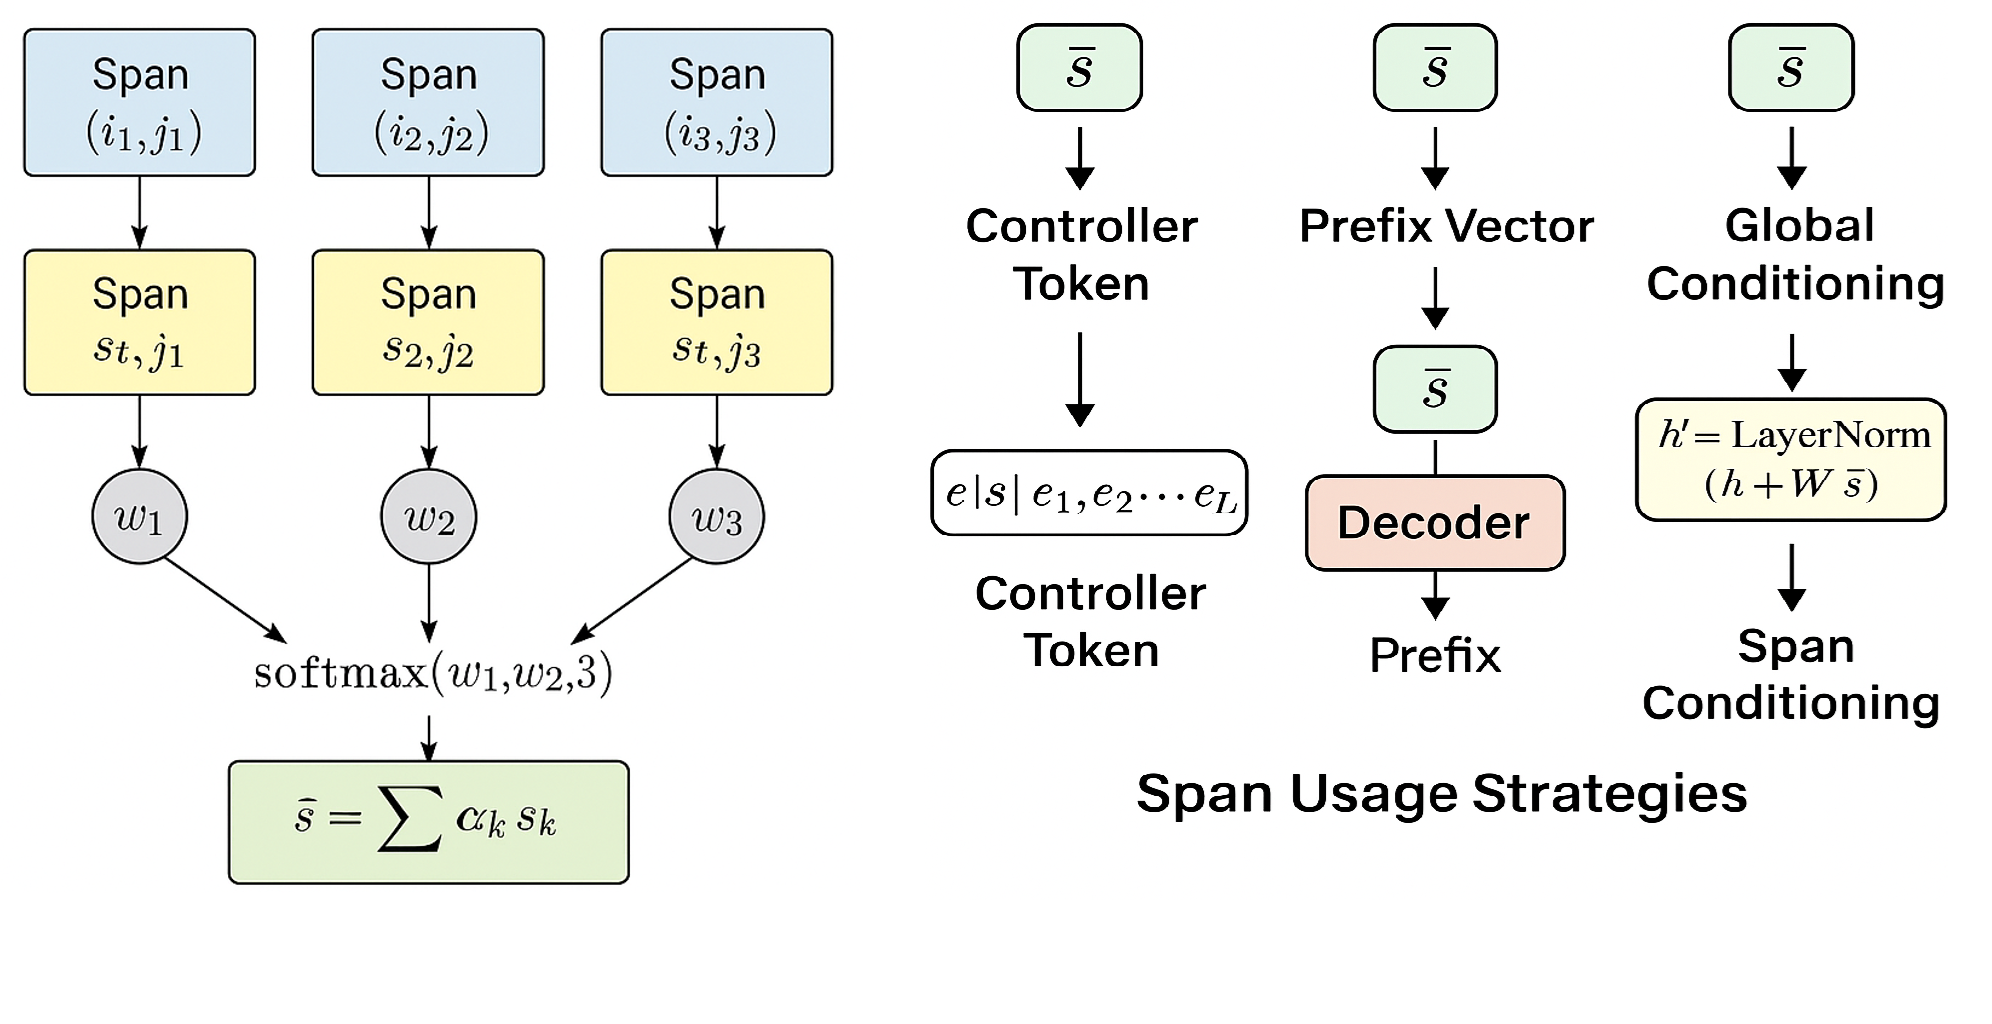
\includegraphics[width=0.95\textwidth]{figures/figure_1.png}
	\caption{Overlap‐aware interpolation of span embeddings.  Each span \(s_k\) is scored by \(w_k\), normalized to \(\alpha_k\), and fused into \(\tilde s\), which then conditions the transformer (Section 3.6).}
	\label{fig:span_interpolation}
\end{figure}

\begin{proposition}[Permutation Equivariance \& Convexity]
	Let \(\{(s_k,w_k)\}_{k=1}^{K'}\) be any reordered set of span‐logit pairs.  Then:
	\begin{enumerate}
		\item \emph{Permutation equivariant}: \(\tilde s\) is invariant to reordering of \(\{s_k\}\).  
		\item \emph{Differentiable}: gradients flow through both \(w_k\) and \(s_k\).  
		\item \emph{Convex}: \(\tilde s\in\mathrm{conv}\{s_k\}_{k=1}^{K'}\).  
	\end{enumerate}
\end{proposition}
\begin{proof}
	Equivariance follows since the softmax in Equation \ref{eq:span_interp} is order‐invariant.  Differentiability holds by the smoothness of \(f_{\mathrm{score}}\) and the linear combination.  Convexity arises because \(\tilde s\) is a positive‐weighted sum of \(\{s_k\}\) with \(\sum_k\alpha_k=1\).
\end{proof}

\paragraph{Computational Cost}  
Computing all \(w_k\) costs \(O(K'd_f)\) (for an MLP of hidden size \(d_f\)), plus \(O(K')\) for softmax.  The final weighted sum costs \(O(K'd)\).  Since \(K'\) is kept small by length filtering and top-\(K\) selection, this interpolation is efficient.

\paragraph{Downstream Integration}  
The fused controller \(\tilde s\) is injected into the transformer as described in Section 3.6 (prefix, attention bias, or gated FFN), enabling full end-to-end learning.